
\section{Simulation numérique}

\subsection{Système étudié}
Pendant les simulations numériques au cas générique on est capable 
d'étudier le système de $N$ satellites (débris) obsérvés par $M$
télescopes. Pour cela on utilise les solutions connues des équations 
de mouvement: 
% \begin{center}
% 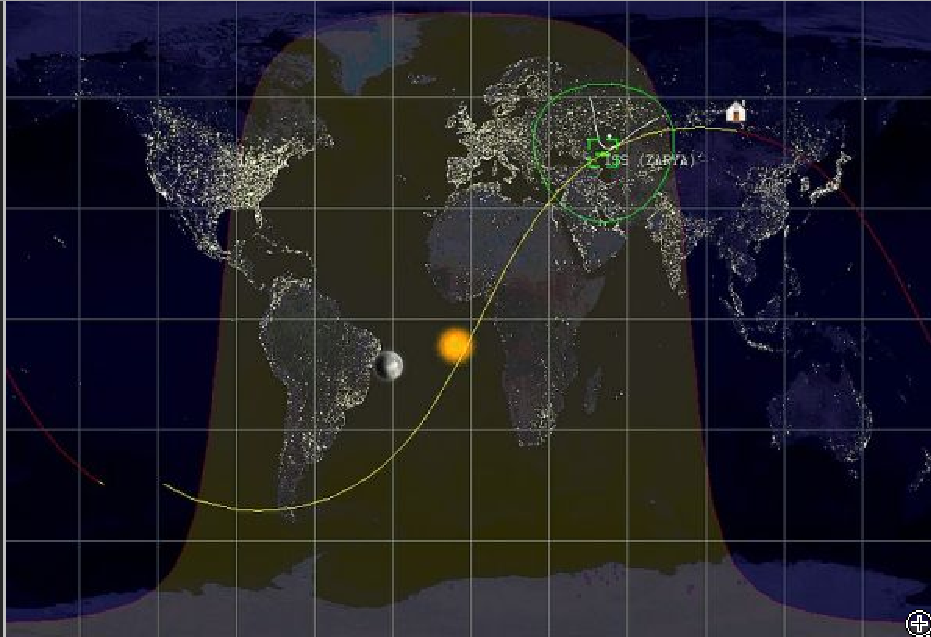
\includegraphics[width = 0.75\linewidth]{map2.pdf} 
% \end{center}
\begin{eqnarray}
   \theta_{O_i}(t) &=& \theta_{O_i}(t_0) + (t-t_0)\dot \theta_{O_i}  \nonumber \\
   \theta_{D_i}(t) &=& \theta_{D_i}(t_0) + (t-t_0)\dot \theta_{D_i} , \, i = 1, \dots N \label{sat} \\
   \theta_{T_j}(t) &=& \theta_{T_j}(t_0) + (t-t_0)\dot \theta_{T_j} , \, j = 1, \dots M \label{tel} \\
   \theta_S(t) &=& \theta_S(t_0) +  (t-t_0)\dot\theta_S  \label{sun} 
\end{eqnarray}
Ici les deux premières éuations sur $\theta_{O_i}$ et $\theta_{D_i}$ caractérisent 
la position de $i$'ème satellite par rapport à un répère fixe; la troisième équation 
sur $\theta_{T_j}$ est expliquée par la rotation de la Terre est caractérise donc 
la position de télescopes; la dernière équation defini l'évaluation de diréction 
du Soleil. 

La trajéctoire typique de satellite (dans un répère fixe) va ``colorer'' une partie de
la sphère
de rayon corréspondant à l'altitude de satellite, ou plus précisement la sphère
sans les ``chapeaux'' autour des pôles, donnés par l'angle d'inclinaison d'orbite. 
Sa projéction sur la Terre qui tourne est donnée sur l'image (\ref{mks})

 \begin{figure}[htp] \centering
     % \includegraphics*[height=3in]{map2.pdf}
      \caption{
            \label{mks}
Projéction de trajéctoire de satellite}
 \end{figure}
 Comme on le voie clairement, la trajéctoire générique n'est pas périodique
 (zone entourée en rouge sur l'image (\ref{mks}))
 

\subsection{La loi de probabilité d'observation}
La première serie des tests numérique a pour but de verifier
l'hypothèse de la loi de probabilité d'observer un satellite 
donnée avec un télescopes donné. 
Comme à chaque instant on connais la position de satellite et de télescope
(éqs. (\ref{sat}, \ref{tel})) on peut comparer ses coordonnées sphèriques 
et conclure si le satellite est dans le champ de vue de télescope. Sur l'image
(\ref{mks}) cette situation corresponde à l'intérsection de projection de
trajectoire avec la zone bleu, representante le télescope.

Le test numérique est donc une simulation de mouvement de $N$ satellites
tous sur l'orbite avec le même angle d'inclinaison $i_d$ de valeure proche (mais pas égale) 
à la valeur correpondante aux satellites héliosynchrones, mais avec une légère difference 
aléatoire de vitesse angulaire et la phase sur l'orbite. Pour le moment on 
ne prende pas en compte les conditions d'écalairage. 

La dépendance de nombre des satellites répérés de temps d'observation
est donnée sur l'image (\ref{proba_obs}). Qualitativement elle corresponde très 
bien à notre estimation théorique. 
 \begin{figure}[htp] \centering
      %\includegraphics*[height=3in]{proba_obs.pdf}
      \caption{
            \label{proba_obs}
  $N = 100$ en vert, $N = 1000$ en rouge, $N = 5000$ en bleu, courbe théorique
  en noir}
 \end{figure}
Ce résultat montre entre autre que l'hypothèse d'indépendence 
d'observer le satellite pendant deux jours consécutifs est 
bien valable au debut d'observation, et que cela change quand
le nombre des satellites déjà répérés devient suffisamment grand.
La difference quantitative entre la probabilité éstimée est simulée
est de 0,XX\%.
  
  
\subsection{Condition d'éclairage et ergodicité}  
Le but de deuxième serie des tests numériques est à la fois de vérifier 
l'independance (moyénne) de condition de visibilité géométrique (position
relative de satellite et de télescope) et d'éclairage (position de
de Soleil) ainsi que étudier l'éffet d'augmentation de nombre des
télescopes. 

% {\small Calcul: cluster de l'ICJ Univ. Claude Bernard Lyon 1}
Le tableau suivant montre le nombre des débris obsérvés
a la fin de simulation pour les differents temps d'observation et nombres des
télescopes.

\begin{center}
\begin{tabular}{|c|c|c|c|} \hline
 Débris & Téléscopes & Temps & \% vus \\ 
 \hline \hline
 100 & 10 & $\sim$ 2 mois &82 \\
 \hline
 100 & 2 & $\sim$ 10 mois &89 \\
 \hline
 \hline
 1000 & 10 & $\sim$ 2 mois &85.5 \\
 \hline
 1000 & 5 & $\sim$ 4 mois &86.7 \\
 \hline
 1000 & 2 & $\sim$ 10 mois &87.7 \\
 \hline  
 \hline
 10000 & 10 & $\sim$ 2 mois &84.0 \\
 \hline
 \hline
 $10^5$ & 14 & $\sim$ 8 mois & $\to 99$ \\
 \hline
\end{tabular} 
\end{center}
  % {\small Calcul: cluster de l'ICJ Univ. Claude Bernard Lyon 1}
Ceci est cohérent avec la probabilité journalière d'observation 
   $p \approx 1\%$, ce qui est bien la valeur estimée suivant l'hypothèse 
   d'indépendence. 
   
   De plus on voie que la probabilité d'observation a la fin de période
   est la même quand le produit de temps d'observation et le nombre des télescopes
   coincide
   
  : ergodicité approximative






